\documentclass[12pt, a4paper]{article}
\usepackage{geometry}
\geometry{margin=1in}
\usepackage{graphicx}
\usepackage{hyperref}
\usepackage{booktabs}
\usepackage{tabularx}
\usepackage{enumitem}
\usepackage{cite}
\usepackage{titlesec}
\usepackage{tikz}
\usetikzlibrary{positioning, shapes.geometric, arrows.meta}

\title{Comprehensive Methods for Microservice Decomposition}
\author{FYP Proposal}
\date{\today}

\begin{document}
\maketitle

\begin{abstract}
This document outlines four highly concrete, distinct methodologies for automated microservice decomposition. Furthermore, \textbf{every single method} has been engineered to strictly fulfill all four primary project objectives (O1: Chunking, O2: Hierarchical Embeddings, O3: Optimization, O4: Tool Development) while maintaining its own unique architectural paradigm.
\end{abstract}

\section{Graph-Contrastive Hierarchical Community Embedding (GC-HCE) Pipeline}

\subsection{Genesis}
\begin{itemize}
    \item \textbf{Sources Consulted:} Citations \cite{jin2021, chaieb2024, bolanowski2022, kalia2020, kalia2021}.
    \item \textbf{Influence:} Citation \cite{jin2021} explicitly suggests clustering the call graph and building hierarchical embeddings. Citations \cite{chaieb2024} and \cite{bolanowski2022} provide the exact metrics (Structural Modularity, Interface Number, ICP) that must be optimized. This method directly translates those theoretical notes into a concrete Graph Neural Network pipeline.
\end{itemize}

\subsection{Objective Coverage}
\begin{itemize}
    \item \textbf{O1 (Chunking):} Employs the Louvain community detection algorithm on the static call graph to identify initial macro-chunks.
    \item \textbf{O2 (Hierarchical Embeddings):} Concatenates macro-embeddings (GraphSAGE representations of communities) with micro-embeddings (CodeBERT vectors of specific functions).
    \item \textbf{O3 (Enhanced Optimization):} Uses a contrastive loss function explicitly weighting Triplet Loss, Structural Modularity (SM), and Inter-partition Communication (ICP) to heavily penalize cross-boundary method calls.
    \item \textbf{O4 (Tool Development):} Packaged as a GitHub Action that parses a repository on commit and generates architectural boundary recommendations in a pull request.
\end{itemize}

\begin{figure}[htbp]
    \centering
    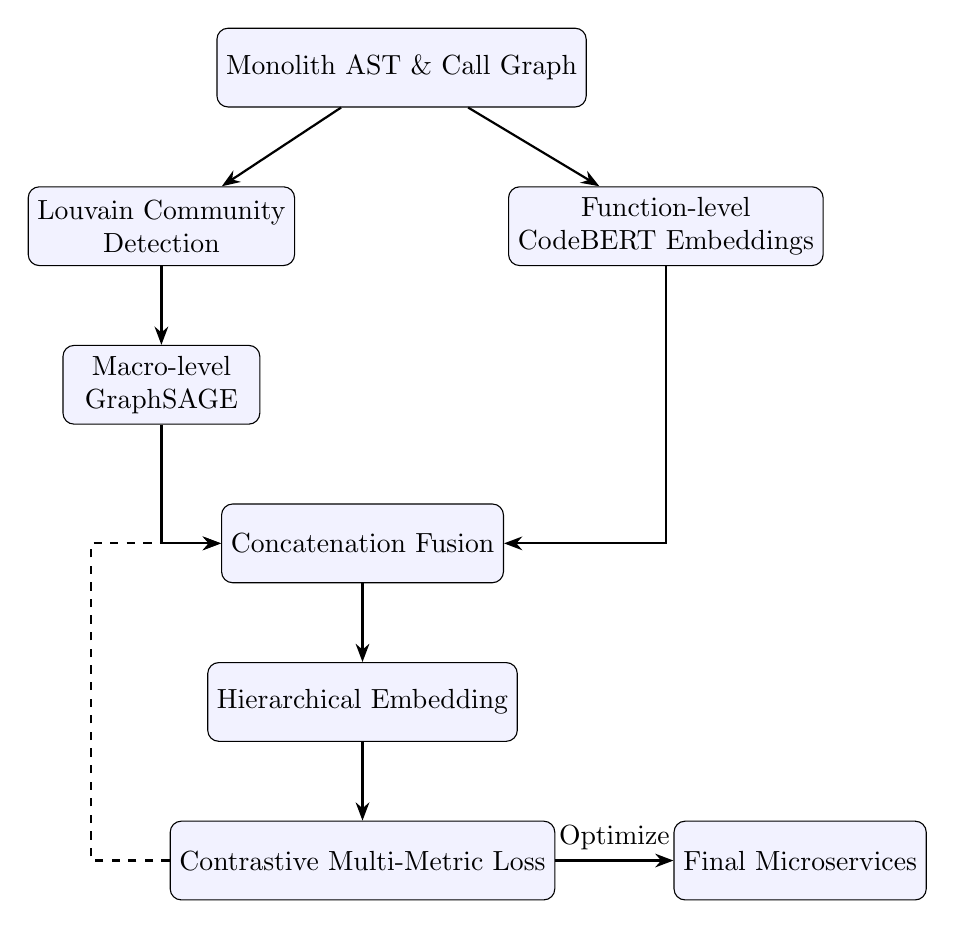
\begin{tikzpicture}[
        box/.style={draw, rectangle, rounded corners, align=center, minimum width=2.5cm, minimum height=1cm, fill=blue!5},
        arrow/.style={->, >=Stealth, thick}
    ]
    \node[box] (ast) {Monolith AST \& Call Graph};
    \node[box, below left=1cm and -1cm of ast] (louvain) {Louvain Community\\Detection};
    \node[box, below right=1cm and -1cm of ast] (codebert) {Function-level\\CodeBERT Embeddings};
    \node[box, below=1cm of louvain] (macro) {Macro-level\\GraphSAGE};
    \node[box, below right=1cm and -0.5cm of macro] (fusion) {Concatenation Fusion};
    \node[box, below=1cm of fusion] (hier) {Hierarchical Embedding};
    \node[box, below=1cm of hier] (loss) {Contrastive Multi-Metric Loss};
    \node[box, right=1.5cm of loss] (services) {Final Microservices};

    \draw[arrow] (ast) -- (louvain);
    \draw[arrow] (ast) -- (codebert);
    \draw[arrow] (louvain) -- (macro);
    \draw[arrow] (macro) |- (fusion);
    \draw[arrow] (codebert) |- (fusion);
    \draw[arrow] (fusion) -- (hier);
    \draw[arrow] (hier) -- (loss);
    \draw[arrow] (loss) -- node[above] {Optimize} (services);
    \draw[arrow, dashed] (loss.west) -- ++(-1,0) |- (fusion.west);
    \end{tikzpicture}
    \caption{Workflow visualization for the GC-HCE Pipeline.}
    \label{fig:gchce}
\end{figure}

\section{Auto-Encoder Driven Multi-Granularity GNN}

\subsection{Genesis}
\begin{itemize}
    \item \textbf{Sources Consulted:} Citations \cite{mathai2022, lin2023, bolanowski2022, kalia2021}.
    \item \textbf{Influence:} Citation \cite{mathai2022} highlights the prior study's use of simple embeddings and the need to combine GNNs. Citation \cite{bolanowski2022} mentions Reconstruction Loss acting as dimensionality reduction. This method builds a two-stream GNN Auto-Encoder to leverage that exact reconstruction mechanism.
\end{itemize}

\subsection{Objective Coverage}
\begin{itemize}
    \item \textbf{O1 (Chunking):} Uses Spectral Clustering on the structural dependency matrix to segment the codebase into highly cohesive initial chunks.
    \item \textbf{O2 (Hierarchical Embeddings):} A two-stream GNN architecture where stream one processes chunk-level macro-nodes and stream two processes class-level micro-nodes, fusing them via a cross-attention mechanism.
    \item \textbf{O3 (Enhanced Optimization):} Focuses heavily on Reconstruction loss combined with Clustering loss and Interface Number (IFN) penalties to ensure decoupled microservices.
    \item \textbf{O4 (Tool Development):} Delivered as a standalone Command Line Interface (CLI) tool capable of ingesting monolithic repositories and exporting decoupled, Docker-ready service definitions.
\end{itemize}

\begin{figure}[htbp]
    \centering
    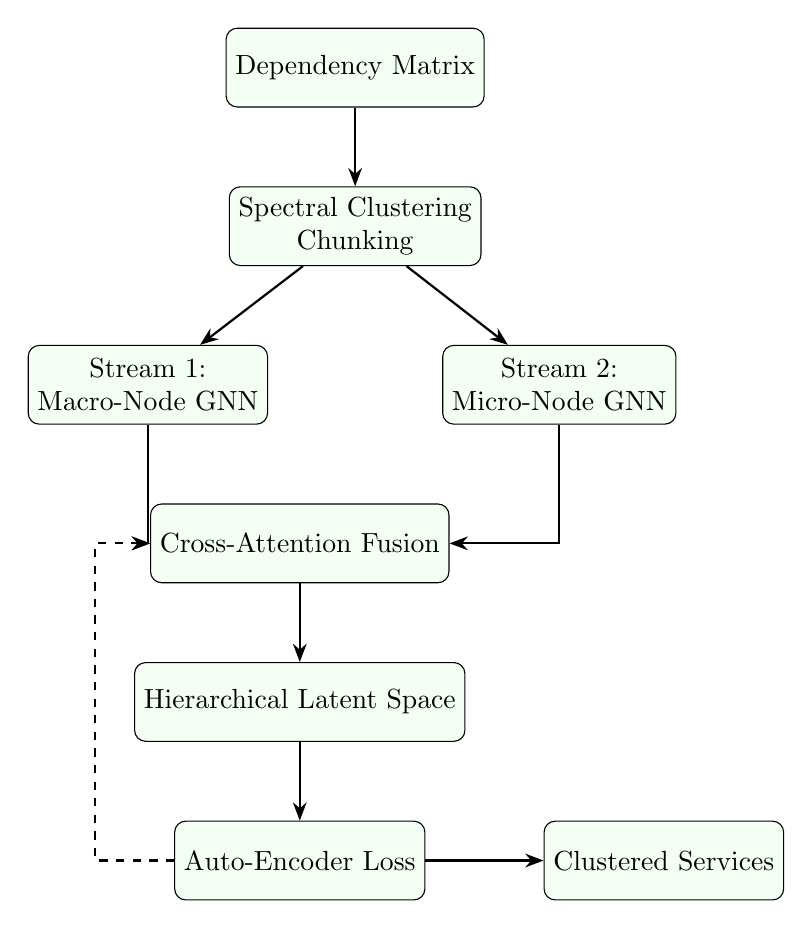
\begin{tikzpicture}[
        box/.style={draw, rectangle, rounded corners, align=center, minimum width=2.5cm, minimum height=1cm, fill=green!5},
        arrow/.style={->, >=Stealth, thick}
    ]
    \node[box] (dep) {Dependency Matrix};
    \node[box, below=1cm of dep] (spec) {Spectral Clustering\\Chunking};
    \node[box, below left=1cm and -0.5cm of spec] (stream1) {Stream 1:\\Macro-Node GNN};
    \node[box, below right=1cm and -0.5cm of spec] (stream2) {Stream 2:\\Micro-Node GNN};
    \node[box, below right=1cm and -1.5cm of stream1] (fusion) {Cross-Attention Fusion};
    \node[box, below=1cm of fusion] (latent) {Hierarchical Latent Space};
    \node[box, below=1cm of latent] (loss) {Auto-Encoder Loss};
    \node[box, right=1.5cm of loss] (services) {Clustered Services};

    \draw[arrow] (dep) -- (spec);
    \draw[arrow] (spec) -- (stream1);
    \draw[arrow] (spec) -- (stream2);
    \draw[arrow] (stream1) |- (fusion);
    \draw[arrow] (stream2) |- (fusion);
    \draw[arrow] (fusion) -- (latent);
    \draw[arrow] (latent) -- (loss);
    \draw[arrow] (loss) -- (services);
    \draw[arrow, dashed] (loss.west) -- ++(-1,0) |- (fusion.west);
    \end{tikzpicture}
    \caption{Workflow visualization for the Auto-Encoder Driven GNN.}
    \label{fig:autoencoder}
\end{figure}

\section{LLM-Bootstrapped Reinforcement Learning Decomposition (RL-MD)}

\subsection{Genesis}
\begin{itemize}
    \item \textbf{Sources Consulted:} Citations \cite{mathai2022, mitchell2007, jin2021, kalia2020}.
    \item \textbf{Influence:} Citation \cite{mathai2022} explicitly states that outputs from decompositions can be used by an LLM-based code generation system to iteratively improve its output. This method formalizes that feedback loop using Reinforcement Learning (RL), where the LLM's feedback and architectural metrics (from \cite{mitchell2007} and \cite{jin2021}) act as the reward signal.
\end{itemize}

\subsection{Objective Coverage}
\begin{itemize}
    \item \textbf{O1 (Chunking):} Leverages structural modularity (SM) maximization directly during the initial code chunking phase using a greedy agglomerative graph approach.
    \item \textbf{O2 (Hierarchical Embeddings):} Stacks semantic embeddings (generated via an LLM for fine-grained functions) on top of structural embeddings (generated via graph algorithms for coarse communities).
    \item \textbf{O3 (Enhanced Optimization):} Replaces standard backpropagation with a Reinforcement Learning agent. The agent adjusts cluster boundaries to maximize a reward function defined exactly by the multi-metric equation: $Reward = SM - IFN - ICP$.
    \item \textbf{O4 (Tool Development):} Built as an interactive web dashboard that connects to GitHub, visualizes the RL agent's boundary shifting process in real-time, and allows architects to manually approve or reject boundaries.
\end{itemize}

\begin{figure}[htbp]
    \centering
    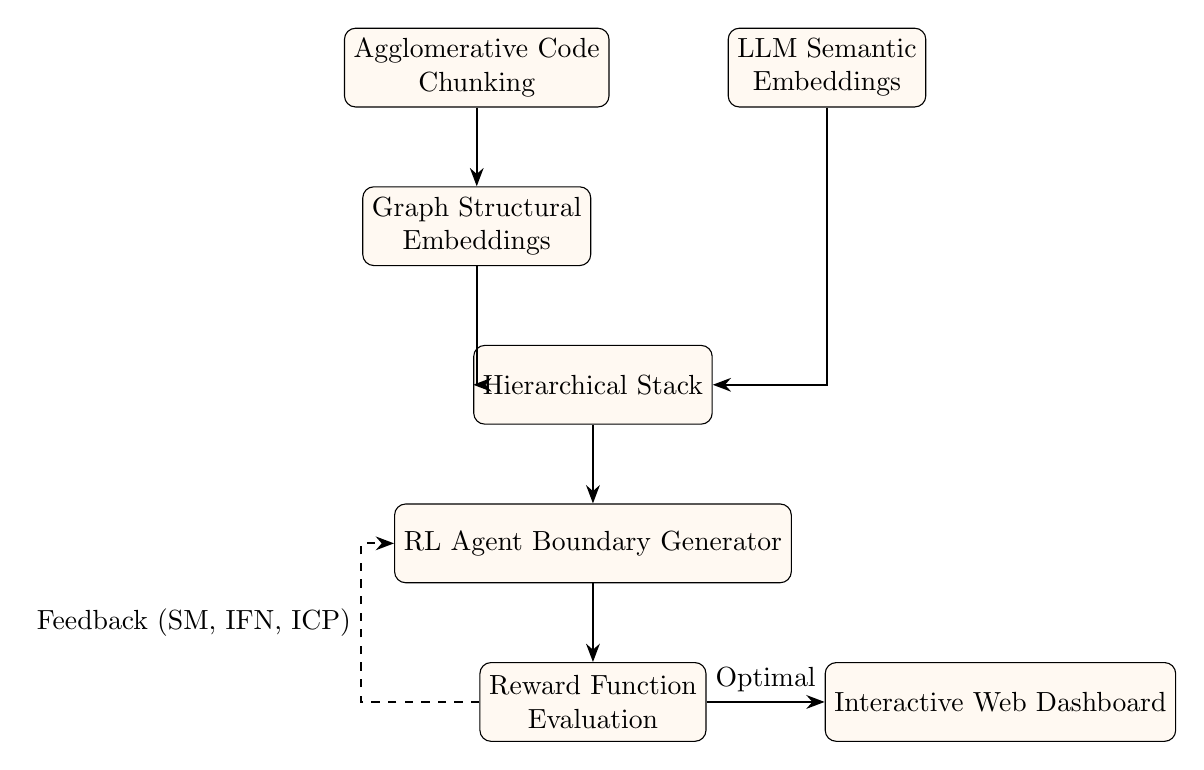
\begin{tikzpicture}[
        box/.style={draw, rectangle, rounded corners, align=center, minimum width=2.5cm, minimum height=1cm, fill=orange!5},
        arrow/.style={->, >=Stealth, thick}
    ]
    \node[box] (agglo) {Agglomerative Code\\Chunking};
    \node[box, right=1.5cm of agglo] (llm) {LLM Semantic\\Embeddings};
    \node[box, below=1cm of agglo] (graph) {Graph Structural\\Embeddings};
    \node[box, below right=1cm and -1.5cm of graph] (stack) {Hierarchical Stack};
    \node[box, below=1cm of stack] (rl) {RL Agent Boundary Generator};
    \node[box, below=1cm of rl] (reward) {Reward Function\\Evaluation};
    \node[box, right=1.5cm of reward] (web) {Interactive Web Dashboard};

    \draw[arrow] (agglo) -- (graph);
    \draw[arrow] (graph) |- (stack);
    \draw[arrow] (llm) |- (stack);
    \draw[arrow] (stack) -- (rl);
    \draw[arrow] (rl) -- (reward);
    \draw[arrow, dashed] (reward.west) -- ++(-1.5,0) |- node[near start, left] {Feedback (SM, IFN, ICP)} (rl.west);
    \draw[arrow] (reward) -- node[above] {Optimal} (web);
    \end{tikzpicture}
    \caption{Workflow visualization for the RL-MD approach.}
    \label{fig:rlmd}
\end{figure}

\section{Adaptive Multi-Metric Contrastive Fusion (AMMCF)}

\subsection{Genesis}
\begin{itemize}
    \item \textbf{Sources Consulted:} Citations \cite{jin2021, kalia2020, chaieb2024, weerasinghe2026}.
    \item \textbf{Influence:} Citation \cite{chaieb2024} introduces the Non-Extreme Distribution (NED) metric used to determine the hyperparameter $k$ (microservice count). This method is directly inspired by making that $k$ calculation dynamic during the training loop, rather than static.
\end{itemize}

\subsection{Objective Coverage}
\begin{itemize}
    \item \textbf{O1 (Chunking):} Implements dynamic call-graph pruning (removing low-weight edges) followed by Girvan-Newman community detection to create highly robust initial chunks.
    \item \textbf{O2 (Hierarchical Embeddings):} Utilizes a dynamic weighting scheme to fuse macro-community embeddings and micro-class embeddings. If a community is highly complex, the model dynamically relies more on the micro-embeddings.
    \item \textbf{O3 (Enhanced Optimization):} Trains via a unified loss function that dynamically scales Triplet loss (for separation) and SM/IFN/ICP (for architectural validity) based on the current epoch's NED score, automatically hunting for the optimum $k$ value.
    \item \textbf{O4 (Tool Development):} Distributed as a VS Code / IDE Extension that provides real-time, on-the-fly decomposition feedback and visualizations for developers working within legacy monoliths.
\end{itemize}

\begin{figure}[htbp]
    \centering
    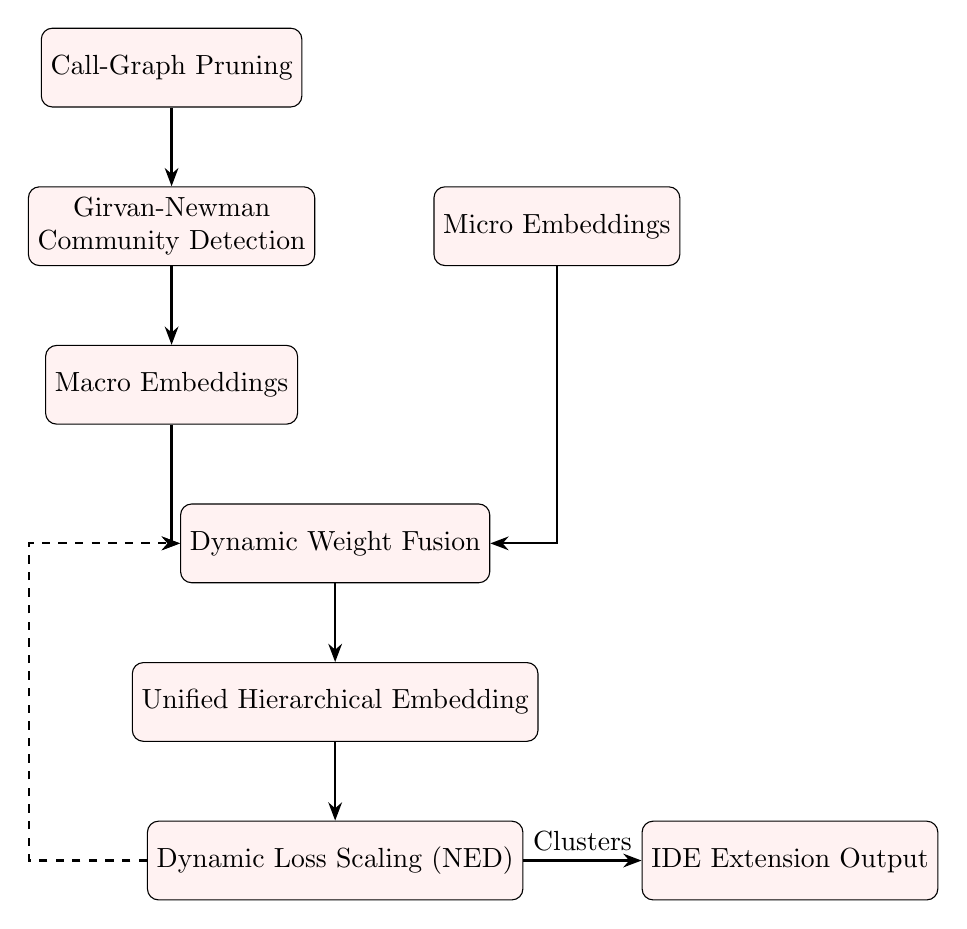
\begin{tikzpicture}[
        box/.style={draw, rectangle, rounded corners, align=center, minimum width=2.5cm, minimum height=1cm, fill=red!5},
        arrow/.style={->, >=Stealth, thick}
    ]
    \node[box] (prune) {Call-Graph Pruning};
    \node[box, below=1cm of prune] (girvan) {Girvan-Newman\\Community Detection};
    \node[box, below=1cm of girvan] (macro) {Macro Embeddings};
    \node[box, right=1.5cm of girvan] (micro) {Micro Embeddings};
    \node[box, below right=1cm and -1.5cm of macro] (fusion) {Dynamic Weight Fusion};
    \node[box, below=1cm of fusion] (unified) {Unified Hierarchical Embedding};
    \node[box, below=1cm of unified] (loss) {Dynamic Loss Scaling (NED)};
    \node[box, right=1.5cm of loss] (ide) {IDE Extension Output};

    \draw[arrow] (prune) -- (girvan);
    \draw[arrow] (girvan) -- (macro);
    \draw[arrow] (macro) |- (fusion);
    \draw[arrow] (micro) |- (fusion);
    \draw[arrow] (fusion) -- (unified);
    \draw[arrow] (unified) -- (loss);
    \draw[arrow] (loss) -- node[above] {Clusters} (ide);
    \draw[arrow, dashed] (loss.west) -- ++(-1.5,0) |- (fusion.west);
    \end{tikzpicture}
    \caption{Workflow visualization for AMMCF.}
    \label{fig:ammcf}
\end{figure}

\bibliographystyle{IEEEtran}
\bibliography{references}

\end{document}
